% \section{Examples}\label{examples}
%
%
% \begin{PW}
% This section presents some sample documents. 
%
% The examples
% in sections~\ref{example:ledfeat} through \ref{example:ledmixed}, plus
% \ref{example:ledbraonain},
% were originally written for TeX.
% I have done some limited conversions of these so that
% they look more like LaTeX code. In particular wherever possible 
% I have replaced \cs{def} commands by either \cs{newcommand} or 
% \cs{renewcommand} as appropriate.
% I have also replaced the original TeX font handling commands by the 
% LaTeX font commands.
%
% The other examples were written natively in LaTeX.
%
%    The figures are from processed versions of the files. Having latexed
% a file I used DVIPS to get Encapsulated PostScript, then the epstopdf
% script to get a PDF version as well, for example: \\
% \begin{verbatim}
% > latex ledeasy
% > latex ledeasy
% > latex ledeasy
% > dvips -E -o ledeasy.eps ledeasy
% > epstopdf ledeasy.eps   % produces ledeasy.pdf
% \end{verbatim}
%
%      For those who aren't fascinated by LaTeX code, I show the all the
% typeset results first, then the code that produced them. 
% 
% \end{PW}
%
% \clearpage
%
% \begin{figure}[p]
% \centering
% 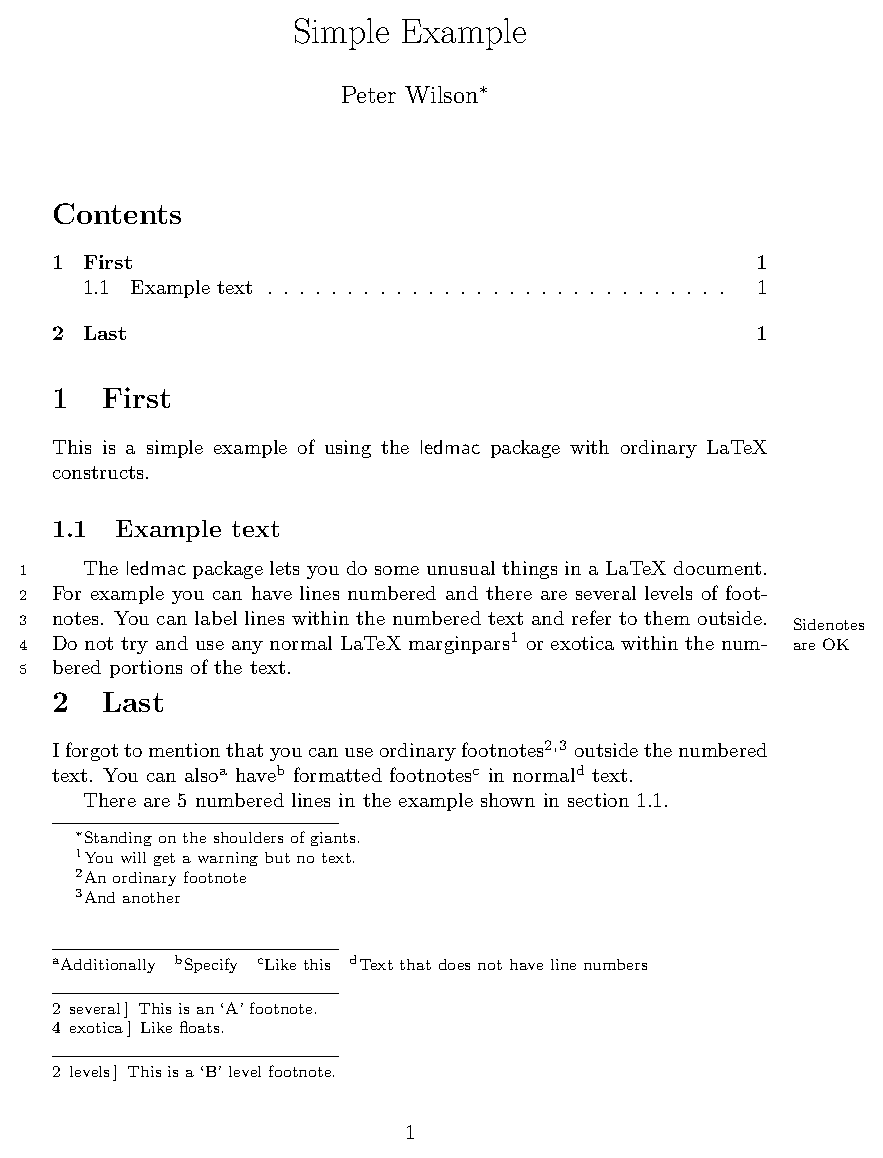
\includegraphics{ledeasy}
% \caption{Output from \file{ledeasy.tex}.}
% \label{easy-out}
% \end{figure}
%
% \begin{figure}[p]
% \centering
% 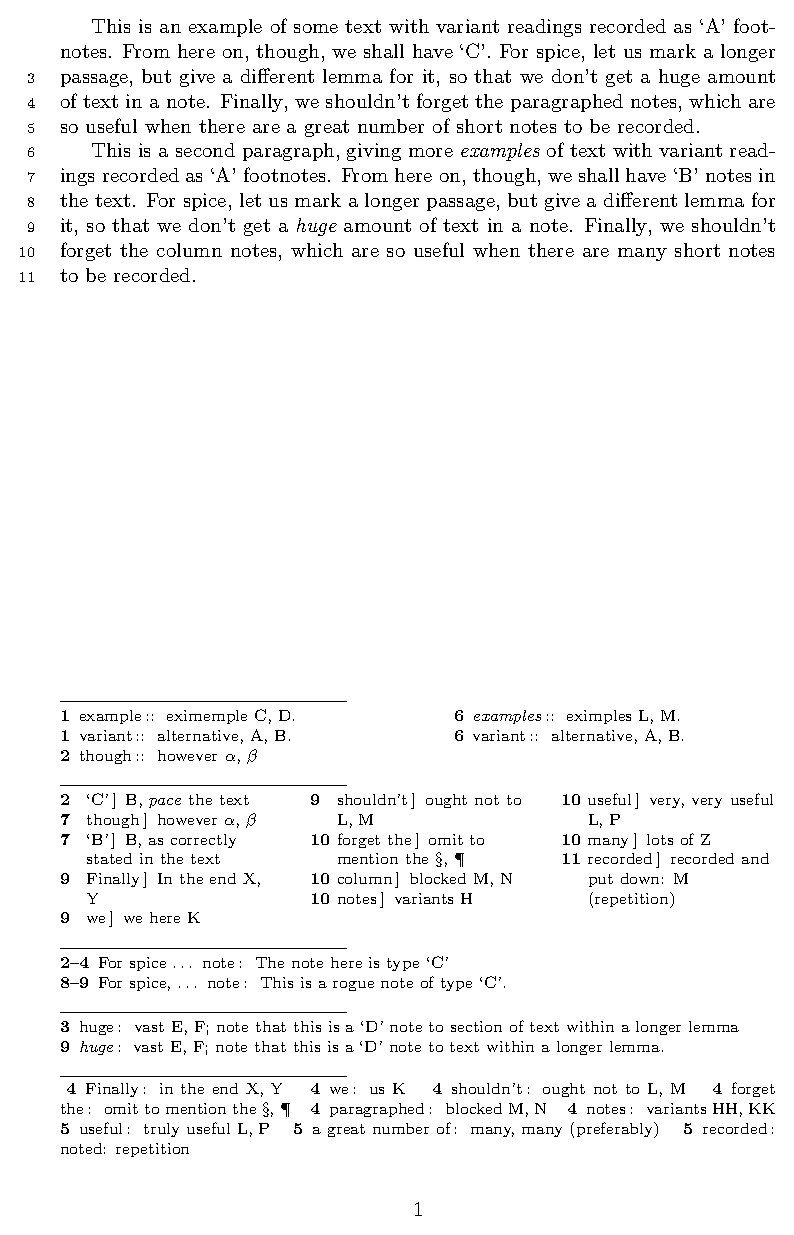
\includegraphics{ledfeat}
% \caption{Output from \file{ledfeat.tex}.}
% \label{features-out}
% \end{figure}
%
% \begin{figure}[p]
% \centering
% 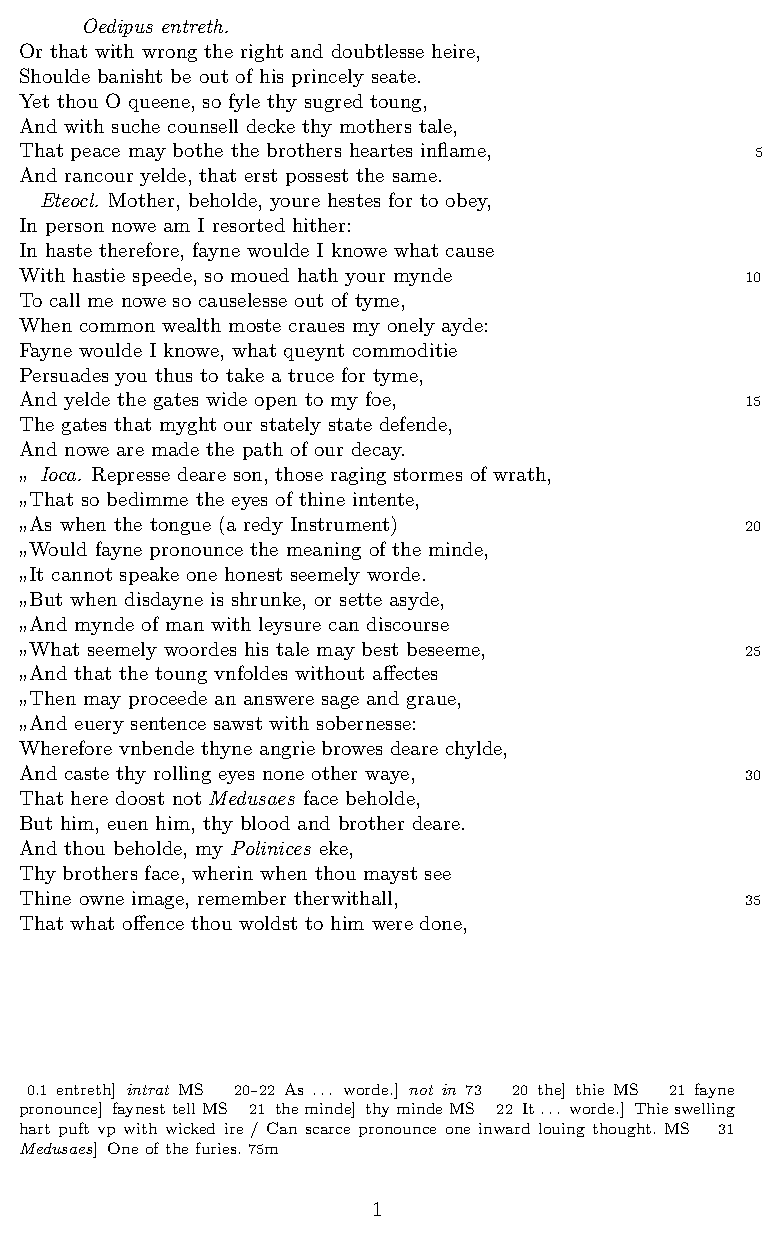
\includegraphics{ledioc}
% \caption{Output from \file{ledioc.tex}.}
% \label{iocasta-out}
% \end{figure}
%
% \begin{figure}[p]
% \centering
% 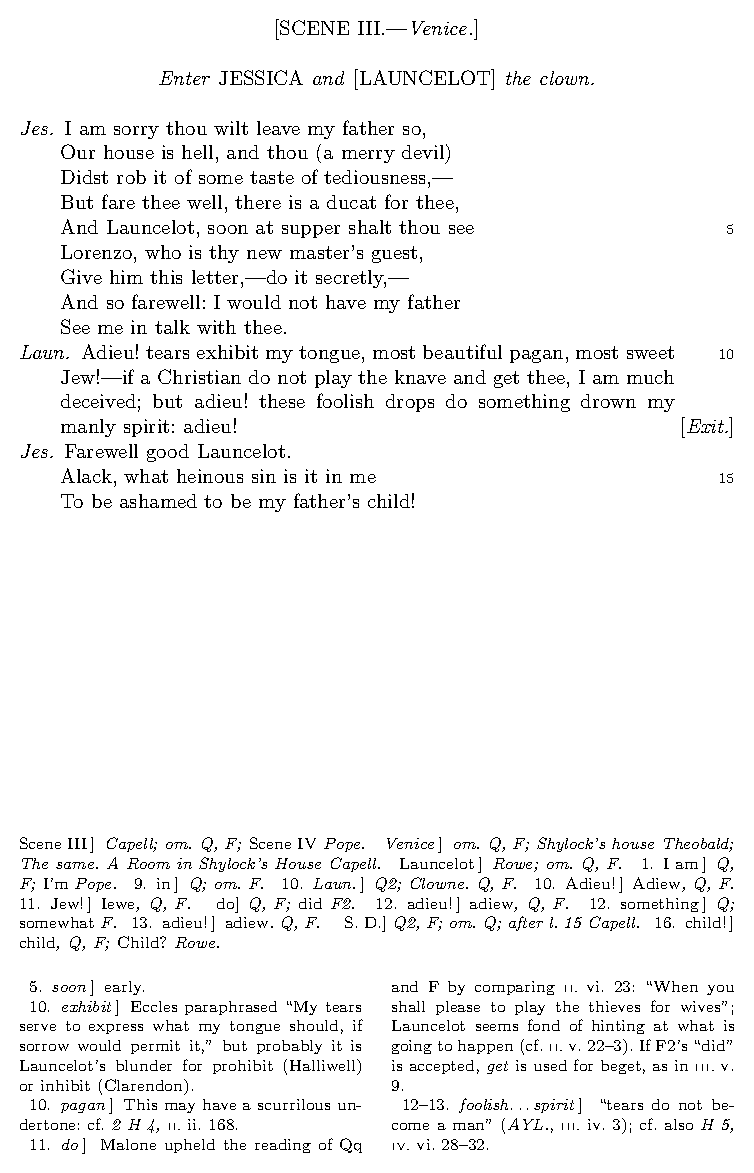
\includegraphics{ledarden}
% \caption{Output from \file{ledarden.tex}.}
% \label{arden-out}
% \end{figure}
%
% \begin{figure}[p]
% \centering
% \hspace*{-2in}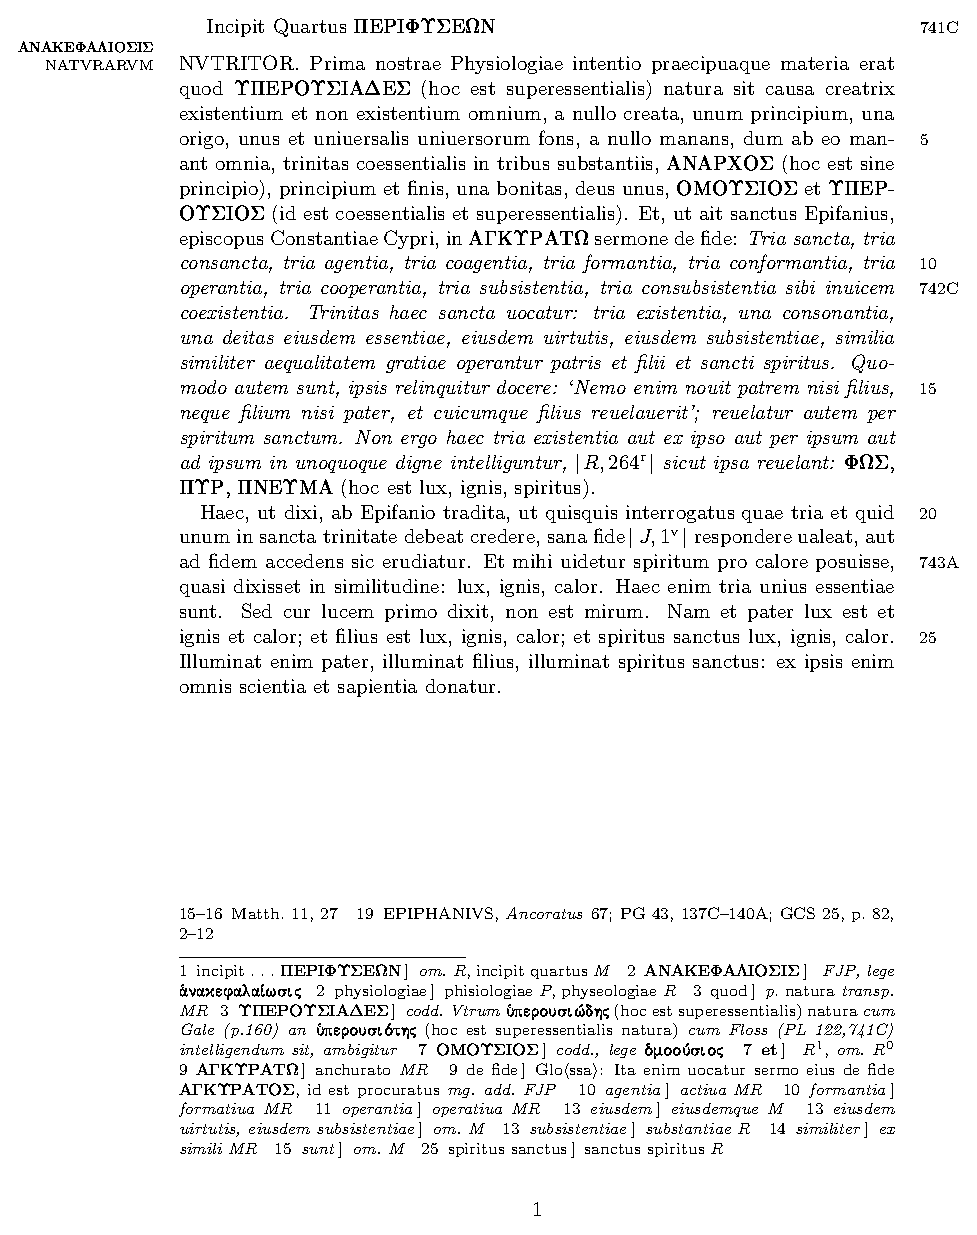
\includegraphics{ledmixed}\hspace*{-2in}
% \caption{Output from \texttt{ledmixed.tex}.}
% \label{periphyseon-out}
% \end{figure}
%
% \begin{figure}[p]
% \centering
% 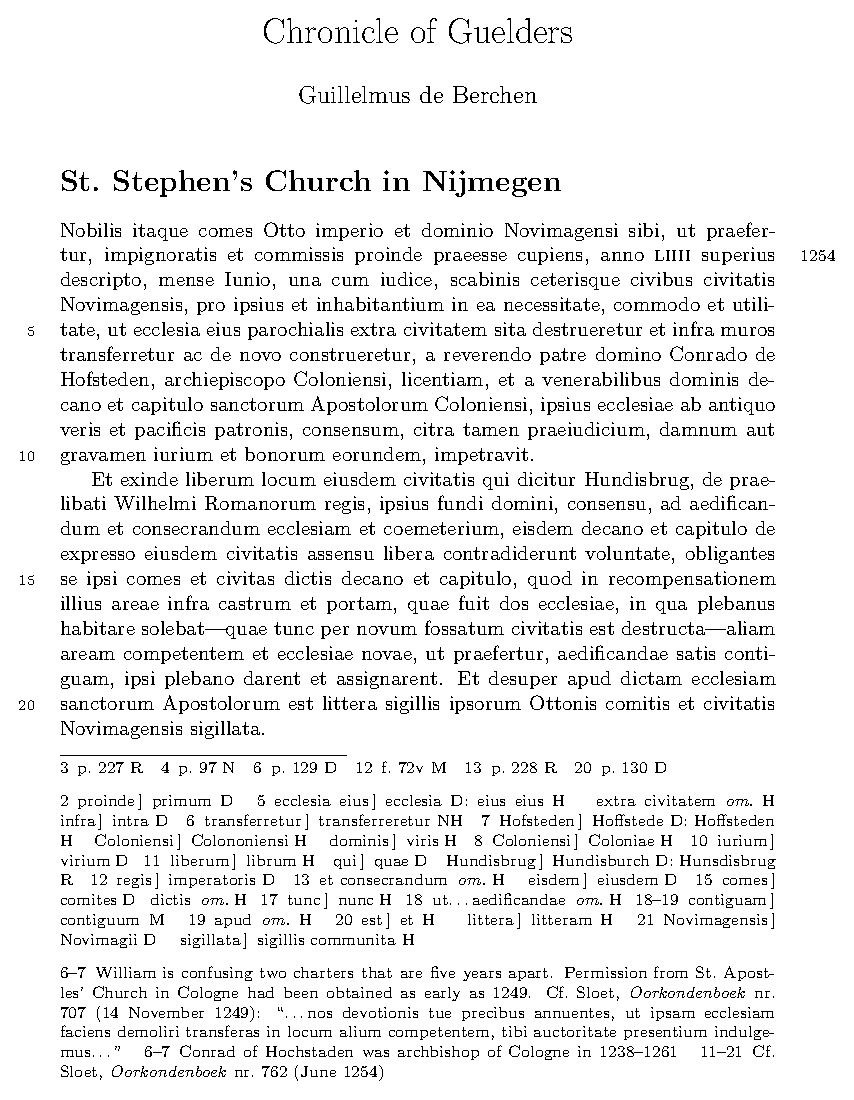
\includegraphics{ledekker}
% \caption{Output from \file{ledekker.tex}.}
% \label{ledekker-out}
% \end{figure}
%
% \begin{figure}[p]
% \centering
% 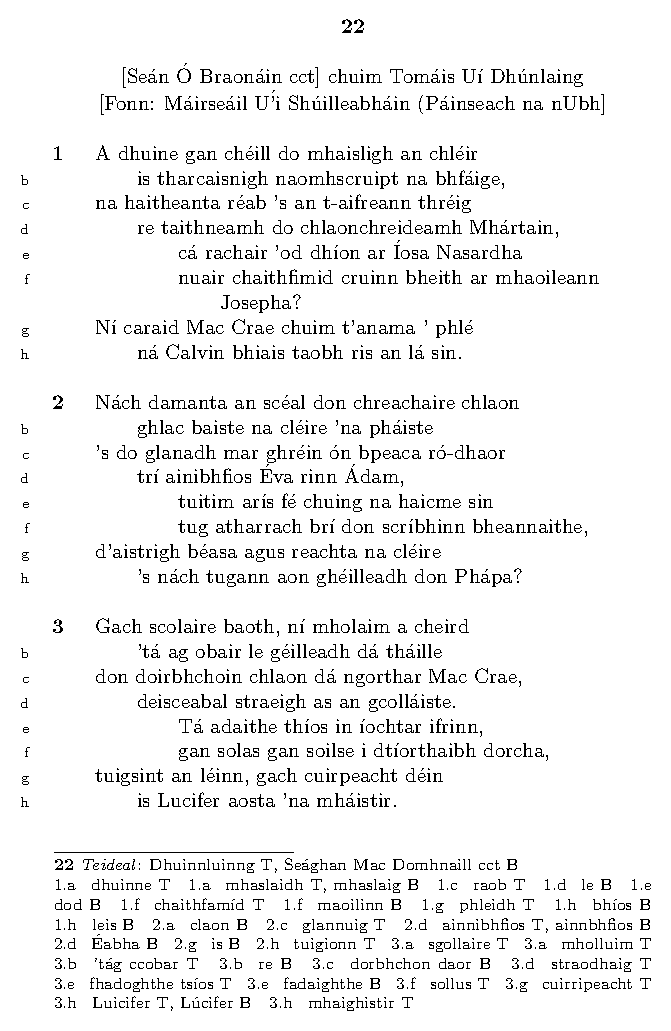
\includegraphics{ledbraonain}
% \caption{Output from \file{ledbraonain.tex}.}
% \label{braonain-out}
% \end{figure}
%
%
% \clearpage
%
% \subsection{Simple example}\label{example:ledeasy}
%
% \begin{PW}
% This made-up example, \file{ledeasy.tex}, is included to show how
% simple it can be to use \edmac{} in a LaTeX document.
% The code is given below and the result is shown in Figure~\ref{easy-out}.
%
% \end{PW}
%
% \medskip
% \hrule
% \medskip
%    \begin{macrocode}
%<*easy>
% ledeasy.tex simple example of the ledmac package
\documentclass{article}
\usepackage{ledmac}
%% number every line
\setcounter{firstlinenum}{1}
\setcounter{linenumincrement}{1}
%% Show some B series familiar footnotes, lettered and paragraphed 
\renewcommand*{\thefootnoteB}{\alph{footnoteB}}
\footparagraphX{B}
%% no endnotes
\noendnotes
%% narrow sidenotes
\setlength{\ledrsnotewidth}{4em}
\title{Simple Example}
\author{Peter Wilson\thanks{Standing on the shoulders of giants.}}
\date{}
\begin{document}
\maketitle
\tableofcontents
\section{First}
   This is a simple example of using the \textsf{ledmac} 
package with ordinary LaTeX constructs.

\subsection{Example text}\label{subsec}

\beginnumbering
\pstart
The \textsf{ledmac} package lets you do some unusual things in
a LaTeX document. For example you can have lines numbered and 
there are  
\edtext{several}{\Afootnote{This is an `A' footnote.}} 
\edtext{levels}{\Bfootnote{This is a `B' level footnote.}}
of footnotes.
You can label lines within the numbered text and refer to them 
outside. Do not try and use any normal LaTeX 
marginpars\footnote{You will get a warning but no text.}%
\ledrightnote{Sidenotes are OK}
or \edtext{exotica}{\Afootnote{Like floats.}}
within the numbered portions of the text\edlabel{line}.
\pend
\endnumbering

\section{Last}

    I forgot to mention that you can use ordinary 
footnotes\footnote{An ordinary footnote}\footnote{And another} 
outside the numbered text. You can also\footnoteB{Additionally}
have\footnoteB{Specify} formatted footnotes\footnoteB{Like this}
in normal\footnoteB{Text that does not have line numbers} text.

   There are \lineref{line} numbered lines in the example shown 
in section~\ref{subsec}.

\end{document}
%</easy>
%    \end{macrocode}
%
%
% \subsection{General example of features} \label{example:ledfeat}
%
% This made-up example, \file{ledfeat.tex}, is included purely to illustrate
% some of \Ledmac's main features.  It is hard to find real-world
% examples that actually use as many layers of notes as this, so we made
% one up.  The example is a bit tricky to read, but close study and
% comparison with the output (Figure~\ref{features-out}) will be
% illuminating.
%
% \begin{PW}
% I have converted the original TeX code to look more like LaTeX code.
% \end{PW}
%
% \medskip
% \hrule
% \medskip
%    \begin{macrocode}
%<*features>
% ledfeat.tex  Small test file for ledmac package
\documentclass{article}
\usepackage{ledmac}

\noendnotes  % we aren't having any endnotes

 \makeatletter
 % I'd like a spaced out colon after the lemma:
 \newcommand{\spacedcolon}{{\rmfamily\thinspace:\thinspace}}
 \renewcommand*{\normalfootfmt}[3]{%
   \ledsetnormalparstuff
   {\notenumfont\printlines#1|}\strut\enspace
   {\select@lemmafont#1|#2}\spacedcolon\enskip#3\strut\par}

 % And I'd like the 3-col notes printed with a hanging indent:
 \renewcommand*{\threecolfootfmt}[3]{%
   \normal@pars
   \hsize .3\hsize
   \setlength{\parindent}{0pt}
   \tolerance=5000       % high, but not infinite
   \raggedright
   \hangindent1.5em \hangafter1
   \leavevmode
   \strut\hbox to 1.5em{\notenumfont\printlines#1|\hfil}\ignorespaces
   {\select@lemmafont#1|#2}\rbracket\enskip
   #3\strut\par\allowbreak}

 % And I'd like the 2-col notes printed with a double colon:
 \newcommand*{\doublecolon}{{\rmfamily\thinspace::\thinspace}}
 \renewcommand*{\twocolfootfmt}[3]{%
   \normal@pars
   \hsize .45\hsize
   \setlength{\parindent}{0pt}
   \tolerance=5000
   \raggedright
   \leavevmode
   \strut{\notenumfont\printlines#1|}\enspace
   {\select@lemmafont#1|#2}\doublecolon\enskip
   #3\strut\par\allowbreak}

 % And in the paragraphed footnotes, I'd like a colon too:
 \renewcommand*{\parafootfmt}[3]{%
   \ledsetnormalparstuff
   {\notenumfont\printlines#1|}\enspace
   {\select@lemmafont#1|#2}\spacedcolon\enskip
   #3\penalty-10 }
 \makeatother

 % I'd like the line numbers picked out in bold.
 \renewcommand{\notenumfont}{\bfseries}
 \lineation{page}
 \linenummargin{inner}
 \setcounter{firstlinenum}{3}       % just because I can
 \setcounter{linenumincrement}{1}
 \foottwocol{A}
 \footthreecol{B}
 \footparagraph{E}
 % I've changed \normalfootfmt, so invoke it again for C and D notes.
 \footnormal{C}
 \footnormal{D}

\begin{document}

 \beginnumbering

 \pstart
 This is an \edtext{example}{
   \Afootnote{eximemple C, D.}}
 of some %\footnote{A normal footnote} 
 text with \edtext{variant}{
   \Afootnote{alternative, A, B.}}
 readings recorded as `A' footnotes.  From here on, \edtext{though}{
   \Afootnote{however $\alpha$, $\beta$}},
 we shall have \edtext{`C'}{
   \Bfootnote{B, \textit{pace} the text}}.
 \edtext{For spice, let us mark a longer passage, but give a different
   lemma for it, so that we don't get a \edtext{huge}{
     \Dfootnote{vast E, F; note that this is
     a `D' note to section of text within a longer lemma}}
   amount of text in a note}{\lemma{For spice \dots\ note}
   \Cfootnote{The note here is type `C'}}.
 \edtext{Finally}{
   \Efootnote{in the end X, Y}},
 \edtext{we}{
   \Efootnote{us K}}
 \edtext{shouldn't}{
   \Efootnote{ought not to L, M}}
 \edtext{forget the}{
   \Efootnote{omit to mention the \S, \P}}
 \edtext{paragraphed}{
   \Efootnote{blocked M, N}}
 \edtext{notes}{
   \Efootnote{variants HH, KK}},
 which are so \edtext{useful}{
   \Efootnote{truly useful L, P}}
 when there are \edtext{a great number of}{
   \Efootnote{many, many (preferably)}}
 short notes to be \edtext{recorded}{
   \Efootnote{noted: repetition}}.
 \pend

 \pstart
 This is a second paragraph, giving more \textit{\edtext{examples}{
   \Afootnote{eximples L, M.}}}
 of text with \edtext{variant}{
   \Afootnote{alternative, A, B.}}
 readings recorded as `A' footnotes.  From here on, \edtext{though}{
   \Bfootnote{however $\alpha$, $\beta$}},
 we  shall have \edtext{`B'}{
   \Bfootnote{B, as correctly stated in the text}} notes in the text.
 \edtext{For spice, let us mark a longer passage, but give a different
   lemma for it, so that we don't get a \textit{\edtext{huge}{
     \Dfootnote{vast E, F; note that this is
     a `D' note to text within a longer lemma.}}}
   amount of text in a note}{\lemma{For spice, \dots\ note}
   \Cfootnote{This is a rogue note of type `C'.}}.
 \edtext{Finally}{
   \Bfootnote{In the end X, Y}},
 \edtext{we}{
   \Bfootnote{we here K}}
 \edtext{shouldn't}{
   \Bfootnote{ought not to L, M}}
 \edtext{forget the}{
   \Bfootnote{omit to mention the \S, \P}}
 \edtext{column}{
   \Bfootnote{blocked M, N}}
 \edtext{notes}{
   \Bfootnote{variants H}},
 which are so \edtext{useful}{
   \Bfootnote{very, very useful L, P}}
 when there are \edtext{many}{
   \Bfootnote{lots of Z}}
 short notes to be \edtext{recorded}{
   \Bfootnote{recorded and put down: M (repetition)}}.
 \pend

 \endnumbering
\end{document}
%</features>
%    \end{macrocode}
% \medskip
% \hrule
% \medskip
%
% \subsection{Gascoigne}
%
% The first real-life example is taken from an edition of George
% Gascoigne's \textit{A Hundreth Sundrie Flowres} that is being
% prepared by G.~W.~Pigman III,\index{Pigman, III$^{rd}$, G. W.} at
% the California Institute of Technology. Figure \ref{iocasta-out}
% shows the result of setting the text with \Ledmac.
%
%
% \begin{PW}
% I have LaTeXified the original code, and removed all the code related
% to the main document layout, relying on the standard LaTeX layout parameters..
% \end{PW}
%
% \medskip
%
% \hrule
% \medskip
%    \begin{macrocode}
%<*ioc>
%% ledioc.tex  
\documentclass{article}
\usepackage{ledmac}

 \noendnotes
 \makeatletter

 \newcommand{\os}{\scriptsize}
 \setcounter{firstsublinenum}{1000}
 \frenchspacing \setlength{\parskip}{0pt} \hyphenpenalty=1000

 % Say \nolinenums if you want no line numbers in the notes.
 \newif\ifnolinenums
 \newcommand{\nolinenums}{\global\nolinenumstrue}
 \newcommand{\linenums}{\global\nolinenumsfalse}

 \renewcommand{\rightlinenum}{\ifbypage@\ifnum\line@num<10\kern.5em\fi\else
 \ifnum\line@num<10\kern1em\else\ifnum\line@num<100
   \kern.5em\fi\fi\fi\kern.5em\numlabfont\the\line@num
   \ifnum\subline@num>0:\the\subline@num\fi}

 \renewcommand{\leftlinenum}{\numlabfont\the\line@num
   \ifnum\subline@num>0:\the\subline@num\fi \kern.5em}
 \linenummargin{outer}
 \lineation{page}

 \newcommand{\ggfootfmt}[3]{%
   \notefontsetup
   \let\par=\endgraf
   \rightskip=0pt \leftskip=0pt
   \setlength{\parindent}{0pt} \parfillskip=0pt plus 1fil
   \ifnolinenums\relax\else
     \begingroup \os \printlines#1|\endgroup
     \enskip
   \fi
   {\rmfamily #2\def\@tempa{#2}\ifx\@tempa\empty
     \else]\enskip\fi#3\penalty-10 }}

 % Now reset the \Afootnote parameters and macros:
 \footparagraph{A}
 \let\Afootfmt=\ggfootfmt
 \dimen\Afootins=\vsize
 \skip\Afootins=3pt plus9pt
 \newcommand*{\ggfootstart}[1]{\vskip\skip\Afootins}
 \let\Afootstart=\ggfootstart

 \newcommand*{\stage}[1]{\pstart\startsub\parindent=0pt
   \hangindent=3em\hangafter=0
   {\itshape #1}\let\par=\finishstage}
 \newcommand{\finishstage}{\pend\endsub}
 \newcommand{\sen}{\leavevmode\lower1ex\hbox{\textrm{''}}}
 \newcommand{\senspeak}[1]{\pstart\obeylines\setbox0=\hbox{\textrm{''}}%
   \leavevmode
   \lower1ex\copy0\kern-\wd0\hskip1em{\textit{#1}}%
   \hbox to1ex{}\ignorespaces}
 \newcommand*{\speak}[1]{\pstart\obeylines\hskip1em{\textit{#1}}%
   \hbox to1ex{}\ignorespaces}
 \def\nospeaker{\parindent=0em\pstart\let\par=\pend}
 \newcommand*{\nospeak}{\pstart\obeylines}
 \makeatother

\begin{document}

 \setlength{\parindent}{0pt}

 \beginnumbering

 \stage{Oedipus \edtext{entreth}{\Afootnote{\textit{intrat} MS}}.}

 \nospeak
 Or that with wrong the right and doubtlesse heire,
 Shoulde banisht be out of his princely seate.
 Yet thou O queene, so fyle thy sugred toung,
 And with suche counsell decke thy mothers tale,
 That peace may bothe the brothers heartes inflame,
 And rancour yelde, that erst possest the same.
 \pend

 \speak{Eteocl.} Mother, beholde, youre hestes for to obey,
 In person nowe am I resorted hither:
 In haste therefore, fayne woulde I knowe what cause
 With hastie speede, so moued hath your mynde
 To call me nowe so causelesse out of tyme,
 When common wealth moste craues my onely ayde:
 Fayne woulde I knowe, what queynt commoditie
 Persuades you thus to take a truce for tyme,
 And yelde the gates wide open to my foe,
 The gates that myght our stately state defende,
 And nowe are made the path of our decay.
 \pend

 \senspeak{Ioca.}Represse deare son, those raging stormes of wrath,
 \sen That so bedimme the eyes of thine intente,
 \edtext{\sen As when \edtext{the}{\Afootnote{thie MS}} tongue %
   (a redy Instrument)
 \sen Would \edtext{fayne pronounce}{\Afootnote{faynest tell MS}} %
   the meaning of \edtext{the minde}{\Afootnote{thy minde MS}},
 \sen \edtext{It}{\lemma{It \dots\ worde.}\Afootnote{Thie %
   swelling hart puft vp with wicked ire / Can scarce pronounce %
   one inward louing thought. MS}} cannot speake one honest %
   seemely worde.}{\lemma{As \dots\ worde.}\Afootnote{\textit{not %
   in} \os73}}
 \sen But when disdayne is shrunke, or sette asyde,
 \sen And mynde of man with leysure can discourse
 \sen What seemely woordes his tale may best beseeme,
 \sen And that the toung vnfoldes without affectes
 \sen Then may proceede an answere sage and graue,
 \sen And euery sentence sawst with sobernesse:
 Wherefore vnbende thyne angrie browes deare chylde,
 And caste thy rolling eyes none other waye,
 That here doost not \edtext{\textit{Medusaes}}{%
 \Afootnote{One of the furies. {\os75}m}} face beholde,
 But him, euen him, thy blood and brother deare.
 And thou beholde, my \textit{Polinices} eke,
 Thy brothers face, wherin when thou mayst see
 Thine owne image, remember therwithall,
 That what offence thou woldst to him were done,
 \pend
 \endnumbering

\end{document}

%</ioc>
%    \end{macrocode}
% \medskip
% \hrule
%
%
% \subsection{Shakespeare} \label{example:ledarden}
%
% The following text illustrates another input file of moderate
% complexity, with two layers of annotation in use. The example is
% taken from the Arden \textit{Merchant of Venice}.\index{Shakespeare, William}
%
%
% \begin{PW}
% I have roughly converted the original TeX file to a LaTeX file.
% The file is below and the result of LaTeXing it is shown in
% Figure~\ref{arden-out}.
% \end{PW}
%
%
% \medskip
% \hrule
% \medskip
%
%    \begin{macrocode}
%<*arden>
%% ledarden.tex
\documentclass{article}
\usepackage{ledmac}

\makeatletter
 \newcommand{\stage}[1]{\rlap{\hbox to \the\linenumsep{%
                        \hfil\llap{[\textit{#1}]}}}}

 \newcommand{\speaker}[1]{\pstart\hangindent2em\hangafter1
   \leavevmode\textit{#1}\enspace\ignorespaces}

 \newcommand{\exit}[1]{\hfill\stage{#1}}

 % LEDMAC customizations:
 \noendnotes
 \setlength{\parindent}{0pt}
 \setlength{\linenumsep}{.4in}
 \rightskip\linenumsep

 \renewcommand{\interparanoteglue}{1em plus.5em minus.1em}

 \newcommand{\scf}{\tiny}
 \let\Afootnoterule=\relax \let\Bfootnoterule=\relax

 \renewcommand{\rightlinenum}{\numlabfont\llap{\the\line@num}}
 \frenchspacing

 % Footnote formats:
 % \nonumparafootfmt is a footnote format without line numbers.
 \newcommand{\nonumparafootfmt}[3]{%
   \ledsetnormalparstuff
   \rightskip=0pt
   \select@lemmafont#1|#2\rbracket\enskip
   \itshape #3\penalty-10 }

 \newcommand{\newparafootfmt}[3]{%
   \ledsetnormalparstuff
   {\notenumfont\printlines#1|}\fullstop\enspace
   {\select@lemmafont#1|#2}\rbracket\enskip
   \itshape #3\penalty-10 }

 \newcommand{\newtwocolfootfmt}[3]{%
   \normal@pars
   \hsize .48\hsize
   \tolerance=5000
   \rightskip=0pt \leftskip=0pt \parindent=5pt
   \strut\notenumfont\printlines#1|\fullstop\enspace
   \itshape #2\/\rbracket\penalty100\hskip .5em plus .5em
   \normalfont #3\strut\goodbreak}

 % Footnote style selections etc. (done last):
 \footparagraph{A}
 \foottwocol{B}
 \let\Afootfmt=\newparafootfmt
 \let\Bfootfmt=\newtwocolfootfmt
 \let\collation=\Afootnote
 \let\note=\Bfootnote
 \lineation{section}
 \linenummargin{right}
 \makeatother

%%%%%%%%%%%%%%%%%%%%%%%%%%%%%%%%

\begin{document}
 \pagestyle{empty}

 % Initially, we don't want line numbers.
 \let\Afootfmt=\nonumparafootfmt

 \beginnumbering
 \pstart
 \centerline{[\edtext{SCENE III}{
   \lemma{Scene III}
   \collation{Capell; om. Q, F; \textnormal{Scene IV} Pope.}}.---%
   \edtext{\textit{Venice}}{
   \collation{om. Q, F; Shylock's house Theobald; The same.
   A Room in Shylock's House Capell.}}.]}
 \pend
 \bigskip

 \pstart
 \centerline{\textit{Enter} JESSICA \textit{and}
   [\edtext{LAUNCELOT}{
   \lemma{Launcelot}
   \collation{Rowe; om. Q, F.}}] \textit{the clown.}} \pend \bigskip

 \let\Afootfmt=\newparafootfmt % we do want line numbers from now

  \setline{0}%

 \speaker{Jes.}\edtext{I am}{
   \collation{Q, F; \textnormal{I'm} Pope.}}
                       sorry thou wilt leave my father so,\\
 Our house is hell, and thou (a merry devil)\\
 Didst rob it of some taste of tediousness,---\\
 But fare thee well, there is a ducat for thee,\\
 And Launcelot, \edtext{soon}{
   \note{early.}}
                        at supper shalt thou see\\
 Lorenzo, who is thy new master's guest,\\
 Give him this letter,---do it secretly,---\\
 And so farewell: I would not have my father\\
 See me \edtext{in}{
   \collation{Q; om. F.}}
              talk with thee.
 \pend

 \speaker{Laun.}
   \edtext{}{\lemma{\textit{Laun.}}\collation{Q2; Clowne. Q, F.}}%
 \edtext{Adieu!}{
   \collation{\textnormal{Adiew}, Q, F.}}
 tears \edtext{exhibit}{
   \note{Eccles paraphrased ``My tears serve to express what my
   tongue should, if sorrow would permit it,'' but probably it is
   Launce\-lot's blunder for prohibit (Halliwell) or inhibit
   (Clarendon).}}
 my tongue, most beautiful \edtext{pagan}{
   \note{This may have a scurrilous undertone: cf. \textit{2 H 4,}
   {\scf II.} \textrm{ii. 168.}}}%
 , most sweet \edtext{Jew!}{
   \collation{\textnormal{Iewe}, Q, F. \quad \textnormal{do]} Q, F;
              \textnormal{did} F2.}}%
 ---if a Christian \edtext{do}{
   \note{Malone upheld the reading of Qq and F by comparing {\scf II.}
    vi. 23: ``When you shall please to play the thieves for
   wives''; Launcelot seems fond of hinting at what is going to
   happen (cf. {\scf II.} v. 22--3). If F2's ``did'' is accepted,
   \textit{get} is used for beget, as in {\scf III.} v. 9.}}
 not play the knave and get thee, I am much deceived; but \edtext{adieu!}{
   \collation{\textnormal{adiew}, Q, F.}}
 these \edtext{foolish drops do \edtext{something}{
   \collation{Q; \textnormal{somewhat} F.}}
 drown my manly spirit}{
   \lemma{foolish\textnormal{\dots}spirit}
   \note{``tears do not become a man'' (\textit{AYL.}, {\scf III.}
   iv. 3); cf. also \textit{H 5,} {\scf IV.} vi. 28--32.}}%
 : \edtext{adieu!}{
   \collation{\textnormal{adiew}. Q, F. \quad \textnormal{S. D.]} Q2, F; om. Q;
   after l. 15 Capell.}}
 \exit{Exit.}
 \pend

 \speaker{Jes.}
 Farewell good Launcelot.\\
 Alack, what heinous sin is it in me\\
 To be ashamed to be my father's \edtext{child!}{
   \collation{\textnormal{child}, Q, F; \textnormal{Child?} Rowe.}}
 \pend
 \endnumbering

\end{document}

%</arden>
%    \end{macrocode}
%
% \medskip
% \hrule
%
%
% \subsection{Classical text edition} \label{example:ledmixed}
%
% The next example, which was extracted from a longer file kindly
% supplied by Wayne Sullivan,\index{Sullivan, Wayne} University
% College, Dublin, Ireland, illustrates the use of \Ledmac{} to
% produce a Latin text edition, the \textit{Periphyseon}, with Greek
% passages.\footnote{The bibliographic details of the forthcoming book
% are: Iohannis Scotti Erivgenae, \textit{Periphyseon} (\textit{De
% Diuisione Naturae}) Liber Qvartvs [Scriptores Latini Hiberniae
% vol.\,xii], (Dublin: School of Celtic Studies, Dublin Institute
% for Advanced Studies, forthcoming 1992).}  The Greek font used is
% that prepared by Silvio Levy\index{Levy, Silvio} and described in 
% \textit{TUGboat}.\footnote{\textit{TUGboat} \textbf{9} (1988), pp.\,20--24.} The
% output of this file is shown in Figure~\ref{periphyseon-out}.
% Note the use of two layers of footnotes to record testimonia and
% manuscript readings respectively.
%
% \begin{PW}
%  I have converted the original \edmac{} example file from TeX
% to something that looks more like LaTeX.
% \end{PW}
%
% ^^A Periphyseon, Liber IV
%
%
% \medskip
% \hrule
% \medskip
%
%    \begin{macrocode}
%<*periph>
% ledmixed.tex
\documentclass{article}
\usepackage{ledmac}

 \noendnotes
%% \overfullrule0 pt
 \lefthyphenmin=3

%    \end{macrocode}
% \begin{PW}
% The LaTeX version uses the \Lpack{lgreek} package to access Silvio Levy's
% greek font. The \texttt{delims} package option 
% subverts\footnote{It actually changes its category code.} the normal meaning
% of \$ to switch in and out of math mode. We have to save the original meaning
% of \$ before calling the package. Later, we use \cs{Ma} and \cs{aM} for math mode
% switching.
% \end{PW}
%    \begin{macrocode}
\let\Ma=$
\let\aM=$
\usepackage[delims]{lgreek}

 % We need an addition to \no@expands since the \active $ in lgreek
 % causes problems:
 \newcommand{\morenoexpands}{\let$=0}

\makeatletter

 \newbox\lp@rbox

 \newcommand{\ffootnote}[2][]{%
   \newcommand{\content}{#2}%
   \ifnumberedpar@
     \xright@appenditem{\noexpand\vffootnote{f}{{\l@d@nums}{\csexpandonce{@tag}}{\csexpandonce{content}}}}%
                                                 \to\inserts@list
     \global\advance\insert@count by 1
 %  \else         %% may be used only in numbered text
 %    \vffootnote{f}{{0|0|0|0|0|0|0}{}{#1}}%
   \fi\ignorespaces}

 \newcommand{\gfootnote}[2][]{%
   \newcommand{\content}{#2}%
   \ifnumberedpar@
     \xright@appenditem{\noexpand\vgfootnote{g}{#1}}%
                                                 \to\inserts@list
     \global\advance\insert@count by 1
 %  \else         %% may be used only in numbered text
 %    \vgfootnote{g}{#1}%
   \fi\ignorespaces}

 \newcommand{\setlp@rbox}[3]{%
   {\parindent\z@\hsize=2.5cm\raggedleft\scriptsize
   \baselineskip 9pt%
   \global\setbox\lp@rbox=\vbox to\z@{\vss#3}}}

 \newcommand{\vffootnote}[2]{\setlp@rbox#2}

 \newcommand{\vgfootnote}[2]{\def\rd@ta{#2}}
 


 \renewcommand{\affixline@num}{%
   \ifsublines@
     \@l@dtempcntb=\subline@num
     \ifnum\subline@num>\c@firstsublinenum
       \@l@dtempcnta=\subline@num
       \advance\@l@dtempcnta by-\c@firstsublinenum
       \divide\@l@dtempcnta by\c@sublinenumincrement
       \multiply\@l@dtempcnta by\c@sublinenumincrement
       \advance\@l@dtempcnta by\c@firstsublinenum
     \else
       \@l@dtempcnta=\c@firstsublinenum
     \fi
     %
     \ifcase\sub@lock
       \or
         \ifnum\sublock@disp=1
            \@l@dtempcntb=0 \@l@dtempcnta=1
         \fi
       \or
         \ifnum\sublock@disp=2 \else
            \@l@dtempcntb=0 \@l@dtempcnta=1
         \fi
       \or
         \ifnum\sublock@disp=0
            \@l@dtempcntb=0 \@l@dtempcnta=1
         \fi
     \fi
   \else
     \@l@dtempcntb=\line@num
     \ifnum\line@num>\c@firstlinenum
        \@l@dtempcnta=\line@num
        \advance\@l@dtempcnta by-\c@firstlinenum
        \divide\@l@dtempcnta by\c@linenumincrement
        \multiply\@l@dtempcnta by\c@linenumincrement
        \advance\@l@dtempcnta by\c@firstlinenum
     \else
        \@l@dtempcnta=\c@firstlinenum
     \fi
     \ifcase\@lock
        \or
          \ifnum\lock@disp=1
             \@l@dtempcntb=0 \@l@dtempcnta=1
          \fi
        \or
          \ifnum\lock@disp=2 \else
             \@l@dtempcntb=0 \@l@dtempcnta=1
          \fi
        \or
          \ifnum\lock@disp=0
             \@l@dtempcntb=0 \@l@dtempcnta=1
          \fi
     \fi
   \fi
   %
   \ifnum\@l@dtempcnta=\@l@dtempcntb
     \@l@dtempcntb=\line@margin
     \ifnum\@l@dtempcntb>1
       \advance\@l@dtempcntb by\page@num
     \fi
     \ifodd\@l@dtempcntb
 %      #1\rlap{{\rightlinenum}}%
        \xdef\rd@ta{\the\line@num}%
     \else
       \llap{{\leftlinenum}}%#1%
     \fi
   \else
     %#1%
   \fi
   \ifcase\@lock
   \or
     \global\@lock=2
   \or \or
     \global\@lock=0
   \fi
   \ifcase\sub@lock
   \or
     \global\sub@lock=2
   \or \or
     \global\sub@lock=0
   \fi}

 \lineation{page}
 \linenummargin{right}
 \footparagraph{A}
 \footparagraph{B}

\renewcommand{\notenumfont}{\footnotesize}
\newcommand{\notetextfont}{\footnotesize}

 \let\Afootnoterule=\relax
 \count\Afootins=825
 \count\Bfootins=825

 \newcommand{\Aparafootfmt}[3]{%
   \ledsetnormalparstuff
   \scriptsize
   \notenumfont\printlines#1|\enspace
 %      \lemmafont#1|#2\enskip
   \notetextfont
   #3\penalty-10\hskip 1em plus 4em minus.4em\relax}

 \newcommand{\Bparafootfmt}[3]{%
   \ledsetnormalparstuff
   \scriptsize
   \notenumfont\printlines#1|\enspace
   \select@lemmafont#1|#2\rbracket\enskip
   \notetextfont
   #3\penalty-10\hskip 1em plus 4em minus.4em\relax }
 \makeatother

 \let\Afootfmt=\Aparafootfmt
 \let\Bfootfmt=\Bparafootfmt
 \def\lemmafont#1|#2|#3|#4|#5|#6|#7|{\scriptsize}
 \parindent=1em

 \newcommand{\lmarpar}[1]{\edtext{}{\ffootnote{#1}}}
 \newcommand{\rmarpar}[1]{\edtext{}{\gfootnote{#1}}}
 \emergencystretch40pt

%%%%%%%%%%%%%%%%%%%%%%%%%%%%%%%%%%%%%%%%%%%%%%

\begin{document}

 \beginnumbering
 \pstart
 \rmarpar{741C}
 \noindent \edtext{Incipit Quartus $PERIFUSEWN$}{%
 \lemma{incipit\ .~.~.\ $PERIFUSEWN$}\Bfootnote{\textit{om.\ R},
 incipit quartus \textit{M}}}
 \pend
 \medskip

 \pstart
 \noindent \edtext{NVTRITOR}{\lemma{$ANAKEFALIOSIS$}\Bfootnote{\textit{
 FJP, lege} $<anakefala'iwsis$}}.\lmarpar{$ANAKEFALIOSIS$
 NATVRARVM} Prima nostrae
 \edtext{Physiologiae}{\lemma{physiologiae}\Bfootnote{phisiologiae
 \textit{P}, physeologiae \textit{R}}} 
 intentio praecipuaque mat\-e\-ria erat 
 \edtext{quod}{\Bfootnote{\textit{p}.\ natura \textit{transp.\ MR}}}
 \edtext{$UPEROUSIADES$}{\Bfootnote{\textit{codd.\ Vtrum}
 $<uperousi'wdhs$ (hoc est superessentialis) natura \textit{cum Gale
 (p.160) an} $<uperousi'oths$ (hoc est superessentialis natura)
 \textit{cum Floss (PL 122,741C) intelligendum sit, ambigitur}}}
 (hoc est superessentialis) natura sit causa creatrix existentium et
 non existentium omnium, a nullo creata, unum principium, una
 origo, unus et uniuersalis uniuersorum fons, a nullo manans, dum
 ab eo manant omnia, trinitas coessentialis in tribus substantiis,
 $ANARQOS$ (hoc est sine principio), principium et finis, una
 bonitas, deus unus, 
 \edtext{$OMOUSIOS$}{\Bfootnote{\textit{codd., lege} $<omoo'usios$}} 
 \edtext{et}{\lemma{\textbf{et}}\Bfootnote{\textit{
 R}\textsuperscript{1}, \textit{om.\ R}\textsuperscript{0}}}
 $UPEROUSIOS$ (id est coessentialis et superessentialis). Et, ut
 ait sanctus Epifanius, episcopus Constantiae Cypri, in
 \edtext{$AGKURATW$}{\Bfootnote{anchurato \textit{MR}}} 
 sermone 
 \edtext{de fide}{\Bfootnote{Glo\Ma\langle\aM ssa\Ma\rangle\aM: Ita
 enim uocatur sermo eius de fide $AGKURATOS$, id est procuratus
 \textit{mg.\ add.\ FJP}}}:
 \begin{itshape}Tria sancta, tria consancta, tria
 \edtext{agentia}{\Bfootnote{actiua \textit{MR}}}, 
 tria coagentia, tria
 \edtext{formantia}{\Bfootnote{formatiua \textit{MR}}}, 
 tria conformantia, tria 
\edtext{operantia}{\Bfootnote{operatiua \textit{MR}}},
 tria cooperantia, tria subsistentia, tria\rmarpar{742C}
 consubsistentia sibi inuicem coexistentia. Trinitas haec
 sancta uocatur: tria existentia, una consonantia, una deitas
 \edtext{eiusdem}{\Bfootnote{eiusdemque \textit{M}}} 
 essentiae,
 \edtext{eiusdem uirtutis, eiusdem
   \edtext{subsistentiae}{\Bfootnote{substantiae \textit{R}}}}{%
 \Bfootnote{\textit{om.\ M}}}, 
 similia 
\edtext{similiter}{\Bfootnote{ex simili \textit{MR}}} 
 aequalitatem gratiae operantur patris et filii et sancti spiritus. 
 Quomodo autem 
 \edtext{sunt}{\Bfootnote{\textit{om.\ M}}}, 
 ipsis relinquitur docere: 
 \edtext{`Nemo enim nouit patrem nisi filius, neque filium nisi pater, 
    et cuicumque filius reuelauerit'}{\Afootnote{Matth.\ 11, 27}}; 
 reuelatur autem per spiritum sanctum. Non ergo haec tria existentia 
 aut ex ipso aut per ipsum aut ad ipsum in unoquoque digne intelliguntur,
 \Ma\mid\! R, 264^{\rm r}\!\mid\aM\ sicut ipsa reuelant:\end{itshape}
 $FWS, PUR, PNEUMA$ 
 \edtext{(hoc est lux, ignis, spiritus)}{\Afootnote{EPIPHANIVS, 
  \textit{Ancoratus} 67; PG~43, 137C--140A; GCS 25, p.~82, 2--12}}.
 \pend

 \pstart
 Haec, ut dixi, ab Epifanio tradita, ut quisquis interrogatus quae
 tria et quid unum in sancta trinitate debeat credere, sana fide
 \Ma\!\mid J, 1^{\rm v}\!\mid\aM\ respondere ualeat, aut ad
 fidem accedens\rmarpar{743A} sic erudiatur. Et mihi uidetur
 spiritum pro calore posuisse, quasi dixisset in similitudine:
 lux, ignis, calor. Haec enim tria unius essentiae sunt. Sed cur
 lucem primo dixit, non est mirum. Nam et pater lux est et ignis
 et calor; et filius est lux, ignis, calor; et 
 \edtext{spiritus sanctus}{\Bfootnote{sanctus spiritus \textit{R}}} 
 lux, ignis, calor. Illuminat enim pater, illuminat filius, illuminat 
 spiritus sanctus: ex ipsis enim omnis scientia et sapientia donatur.
 \pend
 \endnumbering

\end{document}

%</periph>
%    \end{macrocode}
%
% \medskip
% \hrule
%
% ^^A PW: I have removed the bits of the Arabic and Sanskrit examples.
% ^^A PW: the iffalse ... fi trick doesn't work here because of embedded ifs
%
% \subsection{Nijmegen}\label{example:ledekker}
% \changes{v0.2.2}{2003/11/09}{Added the Dekker example}
% \changes{v0.6}{2004/11/16}{Changed version of the Dekker example}
%
% \begin{PW}
% This example, illustrated in Figure~\ref{ledekker-out},
%  was provided in 2004 by Dirk-Jan Dekker\index{Dekker, Dirk-Jan}
% of the Department of Medieval History at the University of 
% Nijmegen\footnote{On 1st September 2004 the University changed its 
% name to Radboud University.}.
% Unlike earlier examples, this was coded for LaTeX and \Ledmac{} from
% the start. I have reformatted the example to help it fit this document;
% any errors are those that I have inadvertently introduced. Note that
% repeated line numbers are eliminated from the footnotes.
% \end{PW}
%
% \medskip
% \hrule
% \medskip
%    \begin{macrocode}
%<*dekker>
%%% This is ledekker.tex, a sample critical text edition
%%% written in LaTeX2e with the ledmac package.
%%% (c) 2003--2004 by Dr. Dirk-Jan Dekker,
%%% University of Nijmegen (The Netherlands)
%%% (PRW) Modified slightly by PRW to fit the ledmac manual

\documentclass[10pt, letterpaper, oneside]{article}
\usepackage[latin]{babel}
\usepackage{ledmac}

\lineation{section}
\linenummargin{left}
\sidenotemargin{outer}

\renewcommand{\notenumfont}{\footnotesize}
\newcommand{\notetextfont}{\footnotesize}

%\let\Afootnoterule=\relax
\let\Bfootnoterule=\relax
\let\Cfootnoterule=\relax

\addtolength{\skip\Afootins}{1.5mm}
%\addtolength{\skip\Bfootins}{1.5mm}
%\addtolength{\skip\Cfootins}{1.5mm}

\makeatletter

\renewcommand*{\para@vfootnote}[2]{%
  \insert\csname #1footins\endcsname
  \bgroup
    \notefontsetup
    \footsplitskips
    \l@dparsefootspec #2\ledplinenumtrue % new from here
    \ifnum\@nameuse{previous@#1@number}=\l@dparsedstartline\relax
      \ledplinenumfalse
     \fi
     \ifnum\previous@page=\l@dparsedstartpage\relax
     \else \ledplinenumtrue \fi
     \ifnum\l@dparsedstartline=\l@dparsedendline\relax
     \else \ledplinenumtrue \fi
     \expandafter\xdef\csname previous@#1@number\endcsname{\l@dparsedstartline}
     \xdef\previous@page{\l@dparsedstartpage} % to here
     \setbox0=\vbox{\hsize=\maxdimen
       \noindent\csname #1footfmt\endcsname#2}%
      \setbox0=\hbox{\unvxh0}%
      \dp0=0pt
      \ht0=\csname #1footfudgefactor\endcsname\wd0
      \box0
      \penalty0
  \egroup
}

\newcommand*{\previous@A@number}{-1}
\newcommand*{\previous@B@number}{-1}
\newcommand*{\previous@C@number}{-1}
\newcommand*{\previous@page}{-1}

\newcommand{\abb}[1]{#1%
        \let\rbracket\nobrak\relax}
\newcommand{\nobrak}{\textnormal{}}
\newcommand{\morenoexpands}{%
        \let\abb=0%
}

\newcommand{\Aparafootfmt}[3]{%
  \ledsetnormalparstuff
  \scriptsize
  \notenumfont\printlines#1|\enspace
%  \lemmafont#1|#2\enskip
  \notetextfont
  #3\penalty-10\hskip 1em plus 4em minus.4em\relax}
        
\newcommand{\Bparafootfmt}[3]{%
  \ledsetnormalparstuff
  \scriptsize
  \notenumfont\printlines#1|%
  \ifledplinenum
      \enspace
  \else
      {\hskip 0em plus 0em minus .3em}
  \fi
  \select@lemmafont#1|#2\rbracket\enskip
  \notetextfont
  #3\penalty-10\hskip 1em plus 4em minus.4em\relax }
       
\newcommand{\Cparafootfmt}[3]{%
  \ledsetnormalparstuff
  \notenumfont\printlines#1|\enspace
%  \lemmafont#1|#2\enskip
  \notetextfont
  #3\penalty-10\hskip 1em plus 4em minus.4em\relax}

\makeatother

\footparagraph{A}
\footparagraph{B}
\footparagraph{C}

\let\Afootfmt=\Aparafootfmt
\let\Bfootfmt=\Bparafootfmt
\let\Cfootfmt=\Cparafootfmt

\emergencystretch40pt

\author{Guillelmus de Berchen}
\title{Chronicle of Guelders}
\date{}
\hyphenation{archi-epi-sco-po Huns-dis-brug li-be-ra No-vi-ma-gen-si}
\begin{document}
\maketitle
\thispagestyle{empty}

\section*{St.\ Stephen's Church in Nijmegen}
\beginnumbering
\autopar

\noindent
Nobilis itaque comes Otto imperio et dominio Novimagensi sibi, 
ut praefertur, impignoratis et commissis 
\edtext{proinde}{\Bfootnote{primum D}} praeesse cupiens, anno 
\textsc{liiii}\ledsidenote{1254} superius descripto, mense 
Iu\edtext{}{\Afootnote{p.\ 227~R}}nio, una cum iudice, scabinis 
ceterisque civibus civitatis Novimagensis, pro ipsius et 
inhabitantium in ea necessitate,\edtext{}{\Afootnote{p.\ 97~N}} 
commodo et utilitate, ut 
\edtext{ecclesia eius}{\Bfootnote{ecclesia D: eius eius H}} 
parochialis 
\edtext{\abb{extra civitatem}}{\Bfootnote{\textit{om.}~H}} sita 
destrueretur et \edtext{infra}{\Bfootnote{intra D}} muros 
\edtext{transfer\edtext{}{\Afootnote{p.\ 129~D}}retur}%
{\Bfootnote{transferreretur NH}} 
ac de novo construeretur, \edtext{a reverendo patre domino 
\edtext{Conrado de \edtext{Hofsteden}%
{\Bfootnote{Hoffstede D: Hoffsteden H}}, 
archiepiscopo 
\edtext{Coloniensi}{\Bfootnote{Colononiensi H}}}%
{\Cfootnote{Conrad of Hochstaden was archbishop of Cologne in 
1238--1261}}, licentiam}{\Cfootnote{William is confusing two 
charters that are five years apart. Permission from St.\ Apostles' 
Church in Cologne had been obtained as early as 1249. Cf.\ Sloet, 
\textit{Oorkondenboek} nr.\ 707 (14 November 1249): 
``\ldots{}nos devotionis tue precibus annuentes, ut ipsam 
ecclesiam faciens demoliri transferas in locum alium competentem, 
tibi auctoritate presentium indulgemus\ldots{}''}}, et a 
venerabilibus \edtext{dominis}{\Bfootnote{viris H}} decano et 
capitulo sanctorum Apostolorum 
\edtext{Coloniensi}{\Bfootnote{Coloniae H}}, ipsius ecclesiae ab 
antiquo veris et pacificis patronis, consensum, citra tamen 
praeiudicium, damnum aut gravamen 
\edtext{iurium}{\Bfootnote{virium D}} et bonorum eorundem, 
impetravit. 

\edtext{Et exinde \edtext{liberum}{\Bfootnote{librum H}} locum 
eiusdem civitatis \edtext{qui}{\Bfootnote{quae D}} dicitur 
\edtext{Hundisbrug}{\Bfootnote{Hundisburch D: Hunsdisbrug R}}, 
de praelibati Wilhelmi Romanorum 
\edtext{regis}{\Bfootnote{imperatoris D}}, ipsius fundi 
do\edtext{}{\Afootnote{f.\ 72v~M}}mini, consensu, ad aedificandum 
\edtext{\abb{et consecrandum}}{\Bfootnote{\textit{om.}\ H}} 
ecclesi\edtext{}{\Afootnote{p.\ 228~R}}am et coemeterium, 
\edtext{eisdem}{\Bfootnote{eiusdem D}} decano et capitulo de 
expresso eiusdem civitatis assensu libera contradiderunt voluntate, 
obligantes se ipsi \edtext{comes}{\Bfootnote{comites D}} et civitas 
\edtext{\abb{dictis}}{\Bfootnote{\textit{om.}\ H}} decano et 
capitulo, quod in recompensationem illius areae infra castrum et 
portam, quae fuit dos ecclesiae, in qua plebanus habitare 
solebat---quae \edtext{tunc}{\Bfootnote{nunc H}} per novum fossatum 
civitatis est destructa---aliam aream competentem et ecclesiae 
novae, 
\edtext{ut praefertur, aedificandae}{\lemma{\abb{ut\ldots aedificandae}}%
\Bfootnote{\textit{om.}\ H}} satis 
\edtext{contiguam}{\Bfootnote{contiguum M}}, ipsi plebano darent 
et assignarent. Et desuper 
\edtext{\abb{apud}}{\Bfootnote{\textit{om.}\ H}} dictam ecclesiam 
sanctorum Apostolorum \edtext{est}{\Bfootnote{et H}} 
\edtext{littera}{\Bfootnote{litteram H}} sigillis ipsorum 
Ottonis\edtext{}{\Afootnote{p.\ 130~D}} comitis et civitatis 
\edtext{Novimagensis}{\Bfootnote{Novimagii D}} 
\edtext{sigillata}{\Bfootnote{sigillis communita H}}.}%
{\Cfootnote{Cf.\ Sloet, \textit{Oorkondenboek} nr.\ 762 (June 1254)}}

% (PRW) the full document continues on after this point
%%%%%%%%%%%%%%%%%%%%%%%%%%%
\endnumbering
\end{document}
%%%%%%%%%%%%%%%%%%

%</dekker>
%    \end{macrocode}
%
% \medskip
% \hrule
% \medskip
%
% \subsection{Irish verse}\label{example:ledbraonain}
% \changes{v0.3}{2004/02/14}{Added the Braonain example}
%
% \begin{PW}
% This example, illustrated in Figure~\ref{braonain-out},
% is a somewhat modified and shortened version of Wayne Sullivan's example 
% demonstration for \edstanza.
%
%  The stanza lines are numbered according to the source verse lines,
% not according to the printed lines. For example, the
% sixth (`f') line in the first stanza is printed as two lines as the source
% line was too long to fit on one printed line. Note that if you process
% this yourself you will get error reports about counters the first time 
% through; this is because alphabetic counters, like roman numerals, have no
% notion of zero.
%
%    As is fairly typical of critical edition typesetting, some of
% \Lpack{ledmac}'s internal macros had to be modified to get the
% desired effects.
% \end{PW}
%
% \medskip
% \hrule
% \medskip
%    \begin{macrocode}
%<*braonain>
%%% This is ledbraonain.tex, a sample critical verse edition.
%%% Originally written for TeX processing with edmac and edstanza
%%% by Wayne Sullivan.
%%% Extensively modified by Peter Wilson for LaTeX and the ledmac package.

\documentclass{article}
\usepackage{ledmac}

\setlength{\textheight}{40pc}
\setlength{\textwidth}{24pc}
\bigskipamount=12pt plus 6pt minus 6pt
\newcommand*{\notetextfont}{\footnotesize}

%%%               Just one footnote series
\footparagraph{C}
\count\Cfootins=800
\makeatletter
%%                but using two different formats
\def\xparafootfmt#1#2#3{%
  \ledsetnormalparstuff
  {\notenumfont\printlines#1|}\enspace
%%%  {\select@lemmafont#1|#2}\rbracket\enskip
       \notetextfont #3\penalty-10 }
\def\yparafootfmt#1#2#3{%
  \ledsetnormalparstuff
%%%  {\notenumfont\printlines#1|}\enspace
%%%  {\select@lemmafont#1|#2}\rbracket\enskip
       \notetextfont #3\penalty-10 }

\let\Cfootfmt=\xparafootfmt
\skip\Cfootins=\bigskipamount
\makeatother

%% This is the default, but just to demonstrate...
\setlength{\stanzaindentbase}{20pt}

%%                  MUST SET THE INDENTS
%% indent multiples; first=hangindent.
%% Must all be non-negative whole numbers
\setstanzaindents{4,1,2,1,2,3,3,1,2,1} 

%%                  Set stanza line penalties
%% Must be nonnegative whole numbers.
%% An initial zero indicates no penalties.
\setstanzapenalties{1,5000,10500,5000,10500,5000,5000,5000,0}
%\setstanzapenalties{0}% the default

%%                   Put some space between stanzas
\let\endstanzaextra=\bigbreak % ==> \bigskip \penalty -200

%% (almost) force line break in foot paragraph
\mathchardef\IMM=9999
\def\lbreak{\hfil\penalty-\IMM} 

%%                   Number each stanza in bold
\newcounter{stanzanum}
\setcounter{stanzanum}{0}
\newcommand*{\numberit}{%
  \flagstanza[0.5\stanzaindentbase]{\textbf{\thestanzanum}}}
%% Use the hook to insert the number (and counteract a new line)
%% and reset the line number to zero
\newcommand*{\startstanzahook}{\refstepcounter{stanzanum}%
  \numberit\vskip-\baselineskip%
  \setlinenum{0}}

%% Want to label the footnotes with the stanza and line number
%% We'll use \linenum to replace the sub-line number
%% with the stanza number, redefining \edtext to do this
%% automatically for us.
%%%%%%%%%%%%%%%%%%%%%%%%%
\makeatletter

\renewcommand{\edtext}[2]{\leavevmode
  \begingroup
    \xdef\@tag{#1}%
    \set@line
    \global\insert@count=0
    \ignorespaces \linenum{||\the\c@stanzanum}#2\relax
    \flag@start
  \endgroup
  #1%
  \ifx\end@lemmas\empty \else
    \gl@p\end@lemmas\to\x@lemma
    \x@lemma
    \global\let\x@lemma=\relax
  \fi
  \flag@end}

%% We need only a very simple macro for footnote numbers,
%% to produce the stanza number (sub-line) then the line number.
\def\printstanzalines#1|#2|#3|#4|#5|#6|#7|{\begingroup
  #3\fullstop \linenumrep{#2}
  \endgroup}
\let\oldprintlines\printlines

\makeatother
%%%%%%%%%%%%%%%%%%%%%%%%%

\pagestyle{empty}

\begin{document}

\beginnumbering

\pstart  \centering \textbf{22}  \pend

\bigskip
%% do not print line number beside heading
\setcounter{firstlinenum}{1000}  
%% and heading footnotes use a different format
\let\Cfootfmt=\yparafootfmt

\pstart
\centerline{[Se\'an \'O Braon\'ain cct] chuim Tom\'ais U\'{\i}
\edtext{Dh\'unlaing}{\Cfootnote{\textbf{22} \textit{Teideal}: Dhuinnluinng T,
Se\'aghan Mac Domhnaill cct B\lbreak}}}
\pend

\pstart
\centerline{[Fonn: M\'airse\'ail U\'{'i} Sh\'uilleabh\'ain (P\'ainseach
             na nUbh]}
\pend

\bigskip

%%           revert to the regular footnote format
\let\Cfootfmt=\xparafootfmt 
%%           but use our special number printing routine
\let\printlines\printstanzalines
%%           Use letters for line numbering
\linenumberstyle{alph}
%%            number lines from the second onwards
\setcounter{firstlinenum}{2}
\setcounter{linenumincrement}{1}

%% Each verse starts with \stanza. 
%% Lines end with &; the last line with \&.

\stanza
A \edtext{dhuine}{\Cfootnote{dhuinne T}} gan ch\'eill do
\edtext{mhaisligh}{\Cfootnote{mhaslaidh T, mhaslaig B}} an chl\'eir&
is tharcaisnigh naomhscruipt na bhf\'aige,&
na haitheanta \edtext{r\'eab}{\Cfootnote{raob T}} 's an 
  t-aifreann thr\'eig&
\edtext{re}{\Cfootnote{le B}} taithneamh do chlaonchreideamh 
  Mh\'artain,&
c\'a rachair \edtext{'od}{\Cfootnote{dod B}} dh\'{\i}on ar 
  \'Iosa Nasardha&
nuair \edtext{chaithfimid}{\Cfootnote{chaithfam\'{\i}d T}} cruinn
bheith ar \edtext{mhaoileann}{\Cfootnote{maoilinn B}} Josepha?&
N\'{\i} caraid Mac Crae chuim t'anama ' 
   \edtext{phl\'e}{\Cfootnote{phleidh T}}&
n\'a Calvin \edtext{bhiais}{\Cfootnote{bh\'{\i}os B}} taobh
\edtext{ris}{\Cfootnote{leis B}} an l\'a sin.\&

\stanza
N\'ach damanta an sc\'eal don chreachaire 
  \edtext{chlaon}{\Cfootnote{claon B}}&
ghlac baiste na cl\'eire 'na ph\'aiste&
's do \edtext{glanadh}{\Cfootnote{glannuig T}} mar ghr\'ein 
  \'on bpeaca r\'o-dhaor&
tr\'{\i} \edtext{ainibhfios}{\Cfootnote{ainnibhfios T, ainnbhfios B}}
\edtext{\'Eva}{\Cfootnote{\'Eabha B}} rinn \'Adam,&
tuitim ar\'{\i}s f\'e chuing na haicme sin&
tug atharrach br\'{\i} don scr\'{\i}bhinn bheannaithe,&
d'aistrigh b\'easa \edtext{agus}{\Cfootnote{is B}} reachta na cl\'eire&
's n\'ach \edtext{tugann}{\Cfootnote{tuigionn T}} aon 
  gh\'eilleadh don Ph\'apa?\&

\stanza
Gach \edtext{scolaire}{\Cfootnote{sgollaire T}} baoth, n\'{\i}
\edtext{mholaim}{\Cfootnote{mholluim T}} a cheird&
\edtext{'t\'a ag obair}{\Cfootnote{'t\'ag ccobar T}} 
  \edtext{le}{\Cfootnote{re B}} g\'eilleadh d\'a th\'aille&
don \edtext{doirbhchoin chlaon}{\Cfootnote{dorbhchon daor B}} 
  d\'a ngorthar Mac Crae,&
deisceabal \edtext{straeigh}{\Cfootnote{straodhaig T}} as an 
  gcoll\'aiste.&
T\'a \edtext{\edtext{adaithe}{\Cfootnote{fadaighthe B}} 
th\'{\i}os}{\Cfootnote{fhadoghthe ts\'{\i}os T}} in 
  \'{\i}ochtar ifrinn,&
gan \edtext{solas}{\Cfootnote{sollus T}} gan soilse i 
  dt\'{\i}orthaibh dorcha,&
tuigsint an l\'einn, gach 
  \edtext{cuirpeacht}{\Cfootnote{cuirripeacht T}} d\'ein&
is \edtext{Lucifer}{\Cfootnote{Luicifer T, L\'ucifer B}} aosta 
  'na \edtext{mh\'aistir}{\Cfootnote{mhaighistir T}}.\&

\endnumbering

\end{document}

%</braonain>
%    \end{macrocode}
%